\documentclass{beamer}

\usepackage[utf8]{inputenc}
\usepackage[greek,english]{babel}
\usepackage{alphabeta}
\usepackage{amsmath}
\usepackage{graphicx}
\usepackage{hyperref}
\usepackage{xcolor}
\usepackage[dvipsnames]{xcolor}

\hypersetup{colorlinks=true, linkcolor=black, urlcolor=black, citecolor=black}

\title{HomeSense: Συλλογή και Οπτικοποίηση Περιβαλλοντικών Δεδομένων με Raspberry Pi}
\author{Ιορδάνης Κωστελίδης}
\date{03/02/2025}
\institute{Πρόγραμμα Μεταπτυχιακών Σπουδών στη Ρομποτική \\
Τμήμα Μηχανικών Πληροφορικής, Υπολογιστών και Τηλεπικοινωνιών \\
Σχολή Μηχανικών \\
Διεθνές Πανεπιστήμιο της Ελλάδος}

\begin{document}

\begin{frame}
\titlepage
\end{frame}

\begin{frame}
\frametitle{Εισαγωγή}
Το \textbf{HomeSense} είναι ένα ολοκληρωμένο σύστημα συλλογής και οπτικοποίησης περιβαλλοντικών δεδομένων, το οποίο βασίζεται στο \textbf{Raspberry Pi 3B+} και σε τρεις ειδικά σχεδιασμένες συσκευές (GasSense, LightSense, TempSense).
\end{frame}

\begin{frame}
\frametitle{Αρχική Σελίδα}
	\centerline{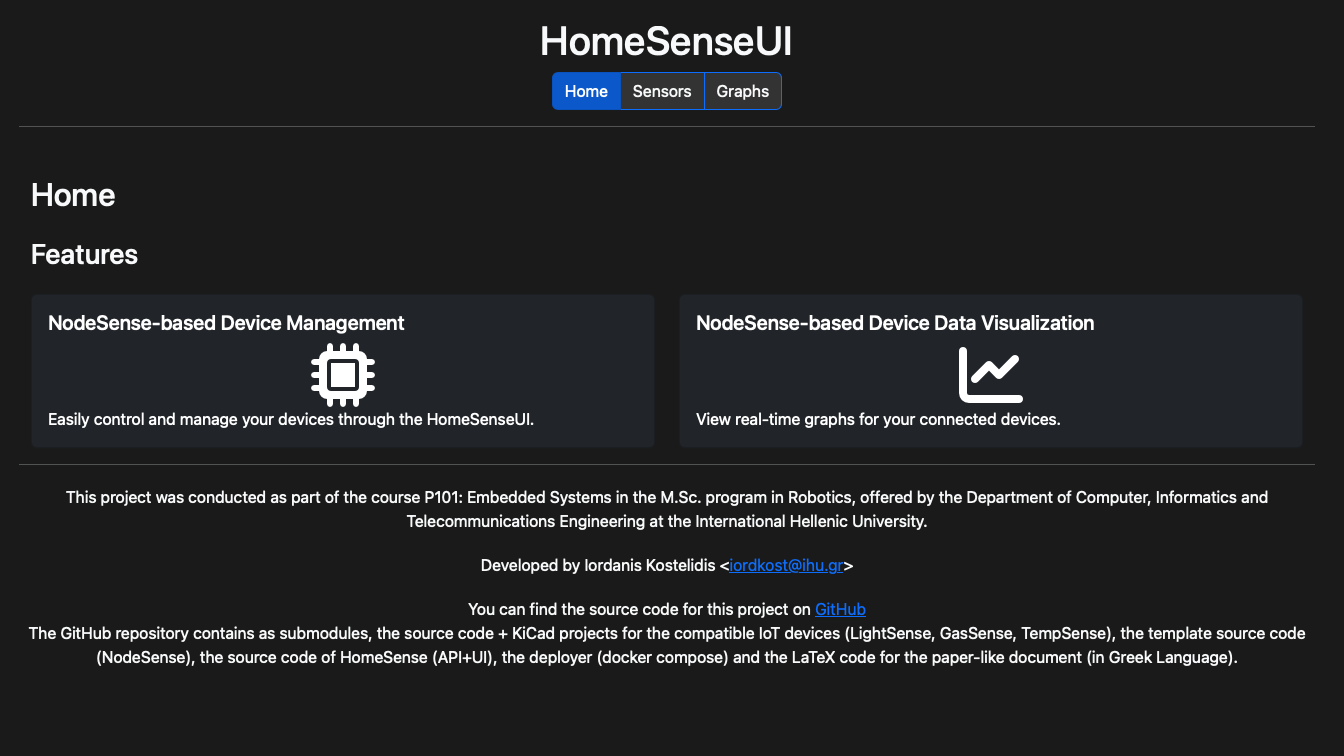
\includegraphics[width=1\textwidth]{assets/index-html}}
\end{frame}

\begin{frame}
\frametitle{Διαχείριση Αισθητήρων}
	\centerline{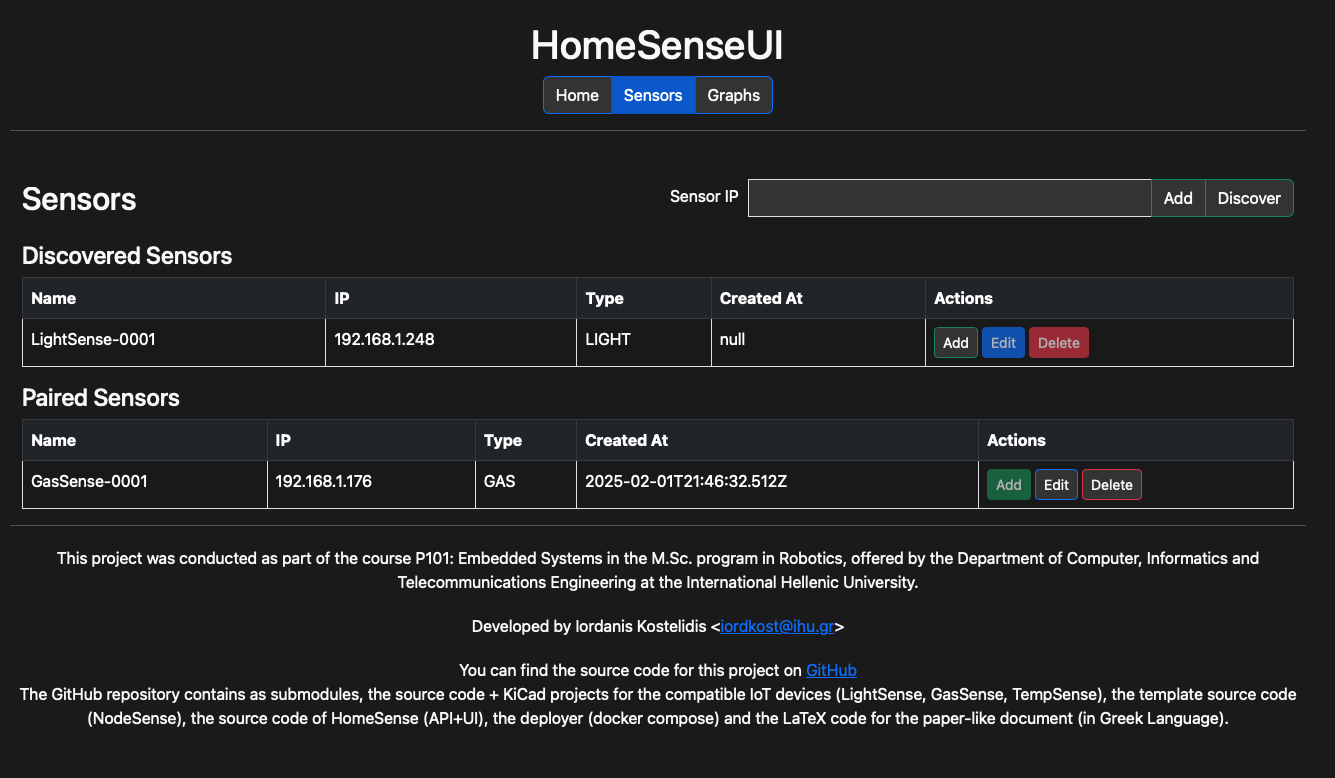
\includegraphics[width=1\textwidth]{assets/sensors-html}}
\end{frame}

\begin{frame}
\frametitle{Γραφήματα}
	\centerline{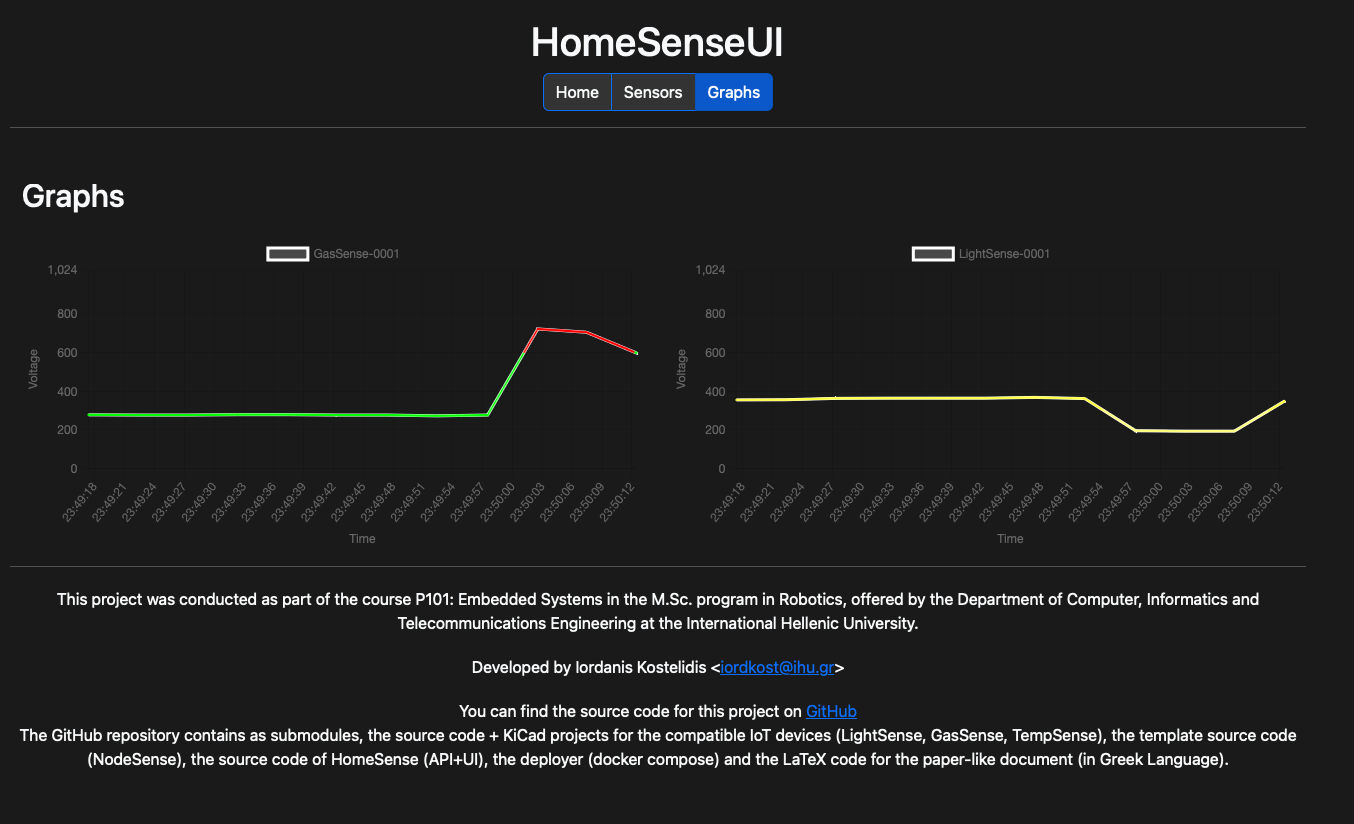
\includegraphics[width=1\textwidth]{assets/graphs-html}}
\end{frame}

\begin{frame}
\frametitle{Αρχιτεκτονική Συστήματος}
\begin{itemize}
    \item \textbf{Raspberry Pi 3B+}: Κεντρικός κόμβος του συστήματος, για συλλογή και αποθήκευση δεδομένων.
    \item \textbf{NodeMCU ESP8266-based Devices}: Τρεις συσκευές που συνδέουν τους αισθητήρες στο δίκτυο Wi-Fi και κάνουν τα δεδομένα διαθέσιμα μέσω HTTP APIs. Οι συσκευές ειναι:
    \begin{itemize}
        \item \textbf{GasSense}: Με MQ-6 (αναλογικός) για την μέτρηση αερίων.
        \item \textbf{LightSense}: Με LDR (αναλογικός) για τη μέτρηση φωτεινότητας.
        \item \textbf{TempSense}: Με DS18B20 (ψηφιακός) για την μέτρηση θερμοκρασίας.
    \end{itemize}
\end{itemize}
\end{frame}

\begin{frame}
\frametitle{Σκοπός του Έργου}
Ο σκοπός του HomeSense είναι:
\begin{itemize}
    \item Η ασύρματη διασύνδεση μικροελεγκτών με ένα Raspberry Pi 3B+ για την καταγραφή και παρουσίαση δεδομένων από τρεις αισθητήρες  
\end{itemize}
\end{frame}

\begin{frame}
\frametitle{Raspberry Pi 3B+}
Το Raspberry Pi 3B+ είναι ο κεντρικός κόμβος του συστήματος, υπεύθυνος για:
\begin{itemize}
    \item Διαχείριση της βάσης δεδομένων.
    \item Εκτέλεση εφαρμογών για την καταγραφή των δεδομένων στην βάση.
    \item Διάθεση διαδικτυακής διεπαφής προς τον χρήστη.
\end{itemize}
\end{frame}

\begin{frame}
\frametitle{NodeSense}
Το NodeSense ειναι ένα template λογισμικό το οποίο είναι συμβατό με τον μικροελεγκτή NodeMCU (ESP8266):
\begin{itemize}
    \item Ορίζει την διαδικασία σύνδεσης με το WiFi
    \item Ορίζει τα Method/Path των HTTP API End-Points
    \item Ορίζει το Response Type των HTTP API End-Points
\end{itemize}
\end{frame}

\begin{frame}
\frametitle{NodeMCU ESP8266-based Devices}
Οι συσκευές (GasSense, LightSense, TempSense) είναι βασισμένες στο λογισμικό NodeSense το οποίο είναι συμβατό με τον μικροελεγκτή NodeMCU (ESP8266):
\begin{itemize}
    \item Το NodeMCU είναι μικρό σε μέγεθος και έχει χαμηλή κατανάλωση ενέργειας.
    \item Έχει εύκολη ενσωμάτωση με το Raspberry Pi (μέσω HTTP API).
    \item Προγραμματίζετε εύκολα με το Arduino IDE, αλλά και με άλλες πλατφόρμες (π.χ. CLion with PlatformIO)
\end{itemize}
\end{frame}

\begin{frame}
\frametitle{GasSense Schematic}
	\centerline{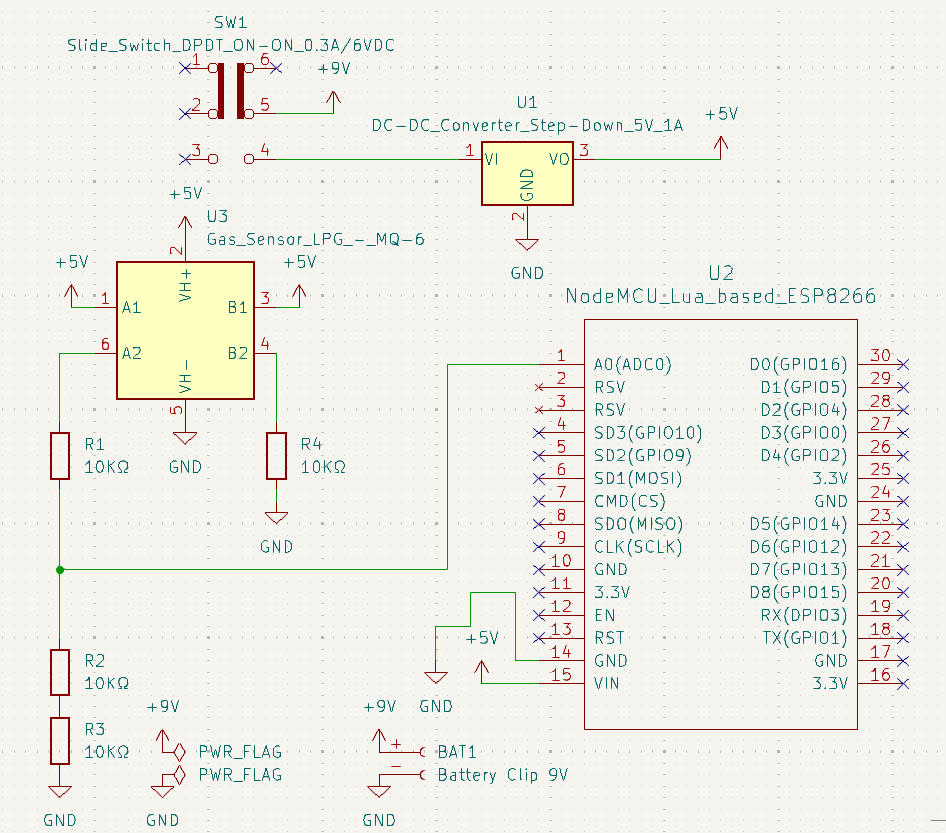
\includegraphics[height=0.6\textwidth]{assets/gassense-schematic}}
\end{frame}
\begin{frame}
\frametitle{GasSense PCB}
	\colorbox{PineGreen}{\centerline{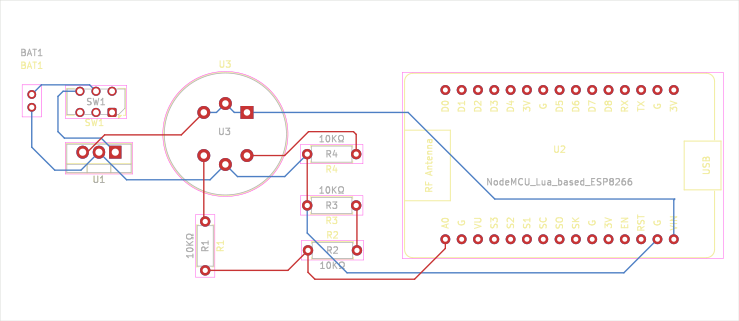
\includegraphics[height=0.4\textwidth]{assets/GasSense-brd}}}
\end{frame}

\begin{frame}
\frametitle{LightSense Schematic}
	\centerline{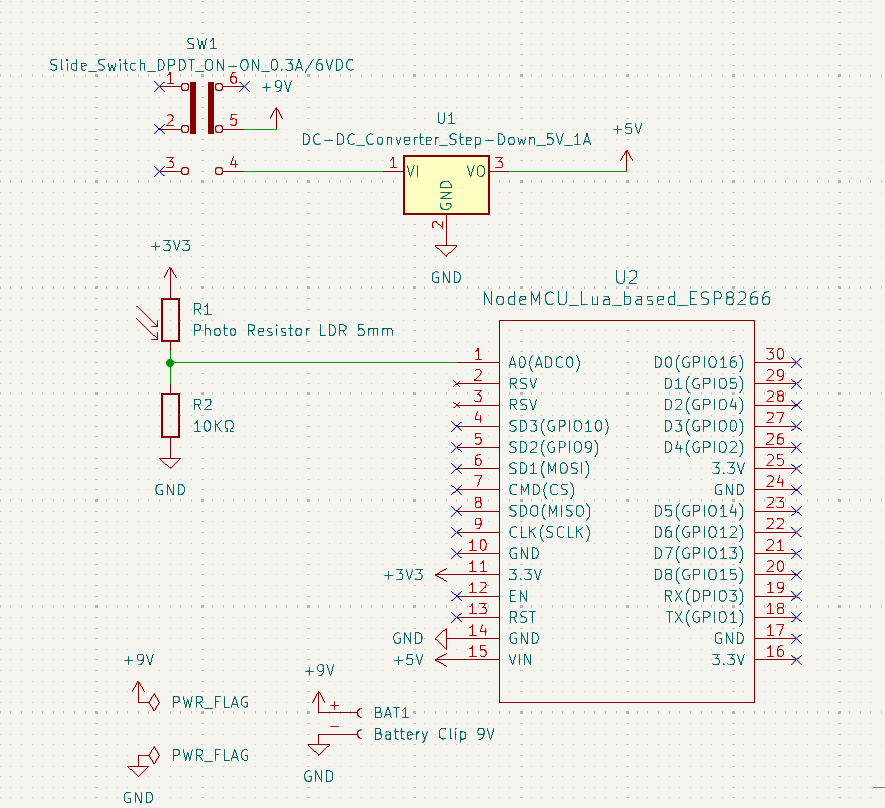
\includegraphics[height=0.6\textwidth]{assets/lightsense-schematic}}
\end{frame}
\begin{frame}
\frametitle{LightSense PCB}
	\colorbox{PineGreen}{\centerline{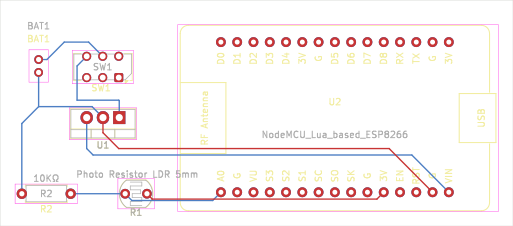
\includegraphics[height=0.4\textwidth]{assets/LightSense-brd}}}
\end{frame}

\begin{frame}
\frametitle{TempSense Schematic}
	\centerline{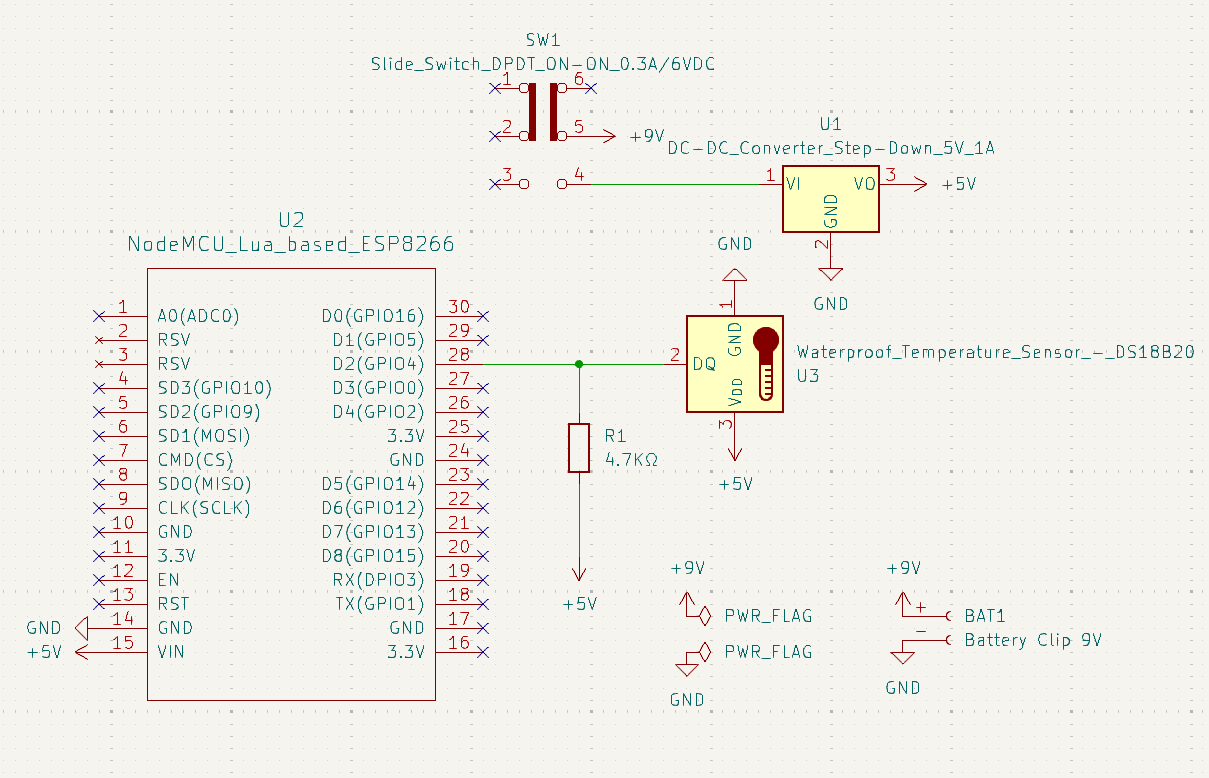
\includegraphics[height=0.6\textwidth]{assets/tempsense-schematic}}
\end{frame}
\begin{frame}
\frametitle{TempSense PCB}
	\colorbox{PineGreen}{\centerline{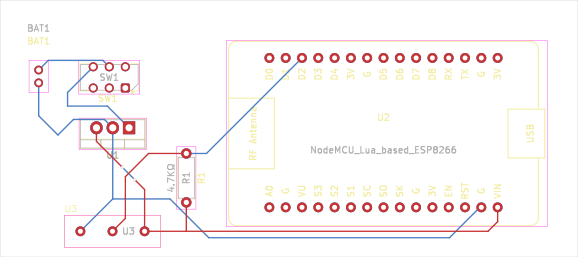
\includegraphics[height=0.4\textwidth]{assets/TempSense-brd}}}
\end{frame}

\begin{frame}
\frametitle{Διαδικασία Συλλογής Δεδομένων}
\begin{itemize}
    \item Ο χρήστης μέσω του UI κάνει pair τις συσκευές με το API.
    \item Το API, κάθε 5 δευτερόλεπτα, κάνει HTTP Call προς τη συσκευή για να λάβει τα δεδομένα του αισθητήρα.
    \item Το API, αποθηκεύει τα δεδομένα σε βάση δεδομένων.
\end{itemize}
\end{frame}

\begin{frame}
\frametitle{Διεπαφή Χρήστη}
\begin{itemize}
    \item Προσθαφαίρεση των συσκευών
    \item Γραφήματα σε πραγματικό χρόνο.
\end{itemize}
\end{frame}

\begin{frame}
\frametitle{It's Demo Time}
DEMO TIME
\end{frame}

\begin{frame}
\frametitle{Εργαλεία και Τεχνολογίες που Χρησιμοποιούνται}
\begin{itemize}
    \item \textbf{Docker}: Πλατφόρμα που επιτρέπει την ανάπτυξη, διανομή και εκτέλεση εφαρμογών μέσα σε απομονωμένα περιβάλλοντα.
    \item \textbf{PostgreSQL}: Βάση δεδομένων για την αποθήκευση δεδομένων.
    \item \textbf{Spring Boot}: Χρησιμοποιείται για την ανάπτυξη του API.
    \item \textbf{HTML/CSS/JavaScript}: Χρησιμοποιείται για την ανάπτυξη του UI.
    \item \textbf{KiCad}: Για τη σχεδίαση των συσκευών (Schematic και PCB).
    \item \textbf{CLion με PlatformIO}: Για την ανάπτυξη του λογισμικού των συσκευών.
    \item \textbf{TeXShop}: Για τη συγγραφή του κειμένου και της παρουσίασης.
\end{itemize}
\end{frame}

\begin{frame}
\frametitle{Μελλοντική Ανάπτυξη}
\begin{itemize}
    \item Επέκταση του συστήματος για την υποστήριξη περισσότερων αισθητήρων.
    \item Επικοινωνία με SSL (HTTPS) για ασφάλεια των δεδομένων.
    \item Αιτήματα μόνο από εξουσιοδοτημένους clients μέσω client-side certificates
    \item Ταυτοποίηση και Εξουσιοδότηση
    \item Ειδοποιήσεις
\end{itemize}
\end{frame}

\begin{frame}
\frametitle{Source Code}
\begin{quote}
Talk is cheap. Show me the code.  
\\ \hfill -- Linus Torvalds
\end{quote}
\end{frame}

\begin{frame}
\frametitle{Source Code}
\begin{quote}
Πόσα repository?
\begin{itemize}
    \item 
\end{itemize}
\end{quote}
\end{frame}

\begin{frame}
\frametitle{Source Code}
\begin{quote}
Πόσα repository?
\begin{itemize}
    \item \textbf{1}?
\end{itemize}
\end{quote}
\end{frame}

\begin{frame}
\frametitle{Source Code}
\begin{quote}
Πόσα repository?
\begin{itemize}
    \item \textbf{1}? ΟΧΙ
\end{itemize}
\end{quote}
\end{frame}

\begin{frame}
\frametitle{Source Code}
\begin{quote}
Πόσα repository?
\begin{itemize}
    \item \textbf{5}?
\end{itemize}
\end{quote}
\end{frame}

\begin{frame}
\frametitle{Source Code}
\begin{quote}
Πόσα repository?
\begin{itemize}
    \item \textbf{5}? ΟΧΙ
\end{itemize}
\end{quote}
\end{frame}

\begin{frame}
\frametitle{Source Code}
\begin{quote}
I don’t have a 'mono-repo' project. I have an ‘ten-repo’ project.
\\ \hfill -- ??? ???
\end{quote}
\end{frame}

\begin{frame}
\frametitle{Source Code}
\begin{quote}
I don’t have a 'mono-repo' project. I have an ‘ten-repo’ project.
\\ \hfill -- Iordanis Kostelidis
\end{quote}
\end{frame}

\begin{frame}
\frametitle{Source Code}
\begin{itemize}
	\item NodeSense: Το αποθετήριο το οποίο περιέχει τον template κώδικα των συσκευών το οποίο βρίσκεται στο \\
	\href{https://github.com/KostelidisDev/NodeSense}{github.com/KostelidisDev/NodeSense}
	\item KiCadGrobotronics: Το αποθετήριο το οποίο περιέχει, custom library για τα components που αγοράστηκαν, από το κατάστημα GRobotronics, το οποίο βρίσκεται στο \\
	\href{https://github.com/KostelidisDev/KiCadGrobotronics}{github.com/KostelidisDev/KiCadGrobotronics}
\end{itemize}
\end{frame}

\begin{frame}
\frametitle{Source Code}
\begin{itemize}
	\item TempSense: Το αποθετήριο το οποίο περιέχει τον κώδικα, το σχηματικό και το PCB της συσκευής με τον αισθητήρα θερμοκρασίας το οποίο βρίσκεται στο \\
	\href{https://github.com/KostelidisDev/TempSense}{github.com/KostelidisDev/TempSense}
	\item LightSense: Το αποθετήριο το οποίο περιέχει τον κώδικα, το σχηματικό και το PCB της συσκευής με τον αισθητήρα φωτός το οποίο βρίσκεται στο \\
	\href{https://github.com/KostelidisDev/LightSense}{github.com/KostelidisDev/LightSense}
	\item GasSense: Το αποθετήριο το οποίο περιέχει τον κώδικα, το σχηματικό και το PCB της συσκευής με τον αισθητήρα αερίου το οποίο βρίσκεται στο \\
	\href{https://github.com/KostelidisDev/GasSense}{github.com/KostelidisDev/GasSense}
\end{itemize}
\end{frame}

\begin{frame}
\frametitle{Source Code}
\begin{itemize}
	\item HomeSense: Το αποθετήριο το οποίο περιέχει τον κώδικα του API και του UI το οποίο βρίσκετε στο \\
	\href{https://github.com/KostelidisDev/HomeSense}{github.com/KostelidisDev/HomeSense}
	\item HomeSense Deployer: Το αποθετήριο το οποίο περιέχει τον deployer για το API και το UI μέσω Docker Compose το οποίο βρίσκεται στο \\
	\href{https://github.com/KostelidisDev/HomeSense-Deployer}{github.com/KostelidisDev/HomeSense-Deployer}
	\item HomeSense-Document: Το αποθετήριο το οποίο περιέχει τον LaTeX κώδικα της εργασίας το οποίο βρίσκεται στο \\
	\href{https://github.com/KostelidisDev/HomeSense-Document}{github.com/KostelidisDev/HomeSense-Document}
	\item HomeSense-Presentation: Το αποθετήριο το οποίο περιέχει τον LaTeX κώδικα της παρουσίασης το οποίο βρίσκεται στο \\
	\href{https://github.com/KostelidisDev/HomeSense-Presentation}{github.com/KostelidisDev/HomeSense-Presentation}
\end{itemize}
\end{frame}

\begin{frame}
\frametitle{Source Code}
\begin{itemize}
	\item HomeSense-Platform: Το κεντρικό αποθετήριο το οποίο έχει ως sub-modules όλα τα σχετικά έργα του HomeSense το οποίο βρίσκεται στο \\
	\href{https://github.com/KostelidisDev/HomeSense-Platform}{github.com/KostelidisDev/HomeSense-Platform}
\end{itemize}
\end{frame}

\begin{frame}
\frametitle{Συμπεράσματα}
Το HomeSense αποτελεί μια ολοκληρωμένη λύση για τη συλλογή και οπτικοποίηση περιβαλλοντικών δεδομένων. 
Με τη χρήση του Raspberry Pi, του NodeMCU και του Docker, προσφέρει ευελιξία, επεκτασιμότητα και αξιοπιστία.
\end{frame}

\begin{frame}
\frametitle{Q\&A}
Ερωτήσεις
\end{frame}

\begin{frame}
\frametitle{}
Ευχαριστώ για την προσοχή σας
\end{frame}

\end{document}